% =====================================================================
% Nanograph: A Structural Graph Representation for Curvilinear Microscopy
% Extended journal version, formatted as a Nature-style submission
% (target: Nature Methods). Uses standard LaTeX packages and the Nature
% bibliography style.
%
% This is an EXPANSION of a MICCAI-style workshop draft into journal length.
% =====================================================================
\documentclass[10pt,a4paper]{article}

\usepackage[T1]{fontenc}
\usepackage{lmodern}
\usepackage[margin=2.5cm]{geometry}
\usepackage{graphicx}
\usepackage{booktabs}
\usepackage{amsmath}
\usepackage{amssymb}
\usepackage{xcolor}
\usepackage{xspace}
\usepackage{microtype}
\usepackage[numbers,sort&compress]{natbib}
\usepackage{authblk}
\usepackage{lineno}
\usepackage{titlesec}
\usepackage[font=small,labelfont=bf]{caption}
\usepackage[hidelinks]{hyperref}

\newcommand{\method}{\textnormal{\textsc{Nanograph}}\xspace}

% Nature-style manuscript typography: compact title block, unnumbered
% headings, bold summary paragraph and continuous line numbering.
% Keep counters active so existing \ref commands remain meaningful, while
% suppressing printed section numbers in the Nature-style headings.
\setcounter{secnumdepth}{3}
\titleformat{\section}{\large\bfseries}{}{0pt}{}
\titleformat{\subsection}{\normalsize\bfseries}{}{0pt}{}
\titleformat{\subsubsection}{\normalsize\itshape}{}{0pt}{}
\titlespacing*{\section}{0pt}{2.2ex plus 0.8ex minus 0.3ex}{0.8ex}
\titlespacing*{\subsection}{0pt}{1.8ex plus 0.6ex minus 0.2ex}{0.5ex}
\renewcommand{\Authfont}{\normalsize}
\renewcommand{\Affilfont}{\small\itshape}
\setlength{\affilsep}{0.5em}
\renewenvironment{abstract}
  {\begin{quote}\small\bfseries\noindent}
  {\end{quote}}
\newenvironment{keywords}
  {\begin{center}\small\textit{Keywords:} }
  {\end{center}}

\begin{document}

\title{Nanograph: A Shape-Preserving Graph Representation of Curvilinear
Structures in High-Content Microscopy}

\author[1]{Nirwan Banerjee\thanks{Correspondence: nirwanbanerjee17@gmail.com}}
\author[1]{Dilip K. Prasad}
\affil[1]{Bio-AI Lab, Department of Computer Science, UiT The Arctic
University of Norway, Troms{\o} 9037, Norway}
\date{}

\maketitle
\linenumbers

\begin{abstract}
High-content and high-throughput microscopy routinely images
\emph{curvilinear} structures---mitochondrial networks, blood vessels,
microtubules and neurites---as dense pixel arrays that are storage-heavy and,
crucially, not structure-aware: downstream morphometric and topological
analysis must re-extract the geometry every time, from scratch and
inconsistently. We present \method, a \emph{shape representation} rather than
a codec: it reduces a curvilinear microscopy image once, faithfully, to an
explicit \emph{attributed graph} whose nodes carry position, width, intensity
and local orientation, and whose edges carry connectivity, length, curvature
and mean width. Because the geometry is made explicit rather than encoded,
morphometry and graph-exact topology ($\beta_0$, $\beta_1$, junction-degree
and network-length statistics) are \emph{read off} the stored object with no
re-processing of pixels, and the image itself can be re-synthesised from the
same object through orientation-aligned point-spread functions. On 726
fluorescence organelle images the representation costs $\approx$\,2.5\,kB per
image and recovers the biological foreground at 28.4\,dB FG-PSNR / 0.997
FG-SSIM relative to its own segmentation mask (27.7\,dB / 0.999 against
independent ground truth). The representation costs essentially the same
storage as the unstructured key-pixel representations it supersedes---the
same budget spent on $3.6\times$ fewer but $3.7\times$ richer
primitives---and it transfers unchanged across five microscopy modalities.
We further analyse the pipeline's dominant bottleneck, foreground
segmentation: a centreline-aware (clDice) U-Net lifts held-out segmentation
IoU from 0.38 to 0.88 in-domain, and a \emph{polarity-agnostic} multi-domain
retraining restores segmentation on four out-of-domain curvilinear
datasets---including electron-microscopy mitochondria, where classical
thresholding scores 0.001 IoU and the retrained network reaches 0.82.
Finally, as evidence that the compactness is genuine rather than an artefact
of discarding structure, we compare against general-purpose codecs at
matched byte budgets. Measured against independent
ground truth, \method is statistically indistinguishable from byte-matched
JPEG on foreground localisation (GT-IoU $0.654$ vs.\ $0.654$; $354/726$ wins,
sign test $p=0.53$, bootstrap 95\% CI on the paired difference
$[-0.0004,+0.0018]$). Its advantage is structural rather than photometric:
the graph's Betti numbers are exact by construction rather than re-estimated
from a decoded array---though their accuracy with respect to the specimen
remains bounded by the foreground segmentation, which we characterise
explicitly---whereas byte-matched JPEG attains a
mean Betti agreement of $0.150\pm0.275$ and inflates $\beta_1$ roughly
eightfold ($4.12\pm3.69$ vs.\ $0.53\pm0.80$); neither codec exposes any
morphometry.
\method extends our own prior line of work on compact image
representation---genetic-algorithm-guided and U-Net-guided key-pixel
selection with kernel- and GAN-based reconstruction---by replacing an
unstructured key-pixel set with an explicit attributed graph and by making
the segmentation front end, previously deferred to future work in that
line, a first-class object of study. In this extended study we
additionally report graph-exact Betti-number topology, quantify the
fidelity contribution of background-grid and residual coding, and document
a case where the pipeline's classical cascade currently out-competes the
more accurate learned segmenter under its default selection heuristic---and
verify that overriding that default lifts in-pipeline segmentation IoU from
0.49 to 0.89 and turns the codec comparison from parity into a significant
ground-truth win, at unchanged payload.
\end{abstract}

\begin{keywords}
Shape representation; Curvilinear structures; Compact image
representation; Graph representation; High-content microscopy;
Segmentation; Topological data analysis
\end{keywords}

% =====================================================================
\section{Introduction}\label{sec:intro}
% =====================================================================
High-content imaging (HCI) and high-throughput screening (HTS) produce vast
collections of microscopy images whose biological content is
\emph{curvilinear}: mitochondrial networks, cytoskeletal filaments, retinal
vasculature and neuronal arbours are all thin, branching, one-dimensional
structures embedded in a two-dimensional (or, in volumetric acquisitions,
three-dimensional) field. Two problems follow from storing such data as raster
images. The first is practical: a single high-content acquisition can reach
gigabyte scale, and generic image codecs (JPEG, WebP, JPEG~2000), tuned for
natural-image statistics, spend most of their bit budget on texture and
background that carry no biological meaning. The second is more fundamental
for analysis: a pixel array is not \emph{structure-aware}. Every downstream
task---branch counting, length and width statistics, connectivity, tracking
across time---must first re-derive the geometry, and does so from scratch and
inconsistently across labs, tools and even repeated runs of the same tool.
It is this second problem that motivates the present work; the first is a
consequence we exploit rather than the objective we optimise.

We argue that the natural representation of a curvilinear microscopy image is a
\emph{graph}. If the structure is reduced once, faithfully, to an attributed
graph---a \emph{nanograph}---then storage, analysis and even approximate image
reconstruction all become downstream reads of the same object. We use the term
deliberately: the attributed graph defined here is the concrete instantiation
of the shape-representation object around which this line of work is
organised, an object that carries complete spatial context in the physical
domain while remaining amenable to scale- and deformation-invariant comparison
in a canonical one. This paper establishes that object and the encoder that
produces it; the homeomorphism-based comparison of nanographs across time, and
the event detection such comparison enables, build directly on the
representation delivered here and are the subject of ongoing work
(Sec.~\ref{sec:discussion}). We instantiate this idea as
\method, an encoder that maps an image to a graph whose nodes are points sampled
along the structural skeleton---each annotated with position, local width,
intensity and tangent orientation---and whose edges encode branch connectivity
together with per-branch morphometry (length, mean width, curvature). From this
graph the image can be re-synthesised by placing \emph{orientation-aligned}
elliptical point-spread functions (PSFs) at the sampled nodes and adding a
low-rank background field plus an optional foreground residual.

This journal version substantially extends a prior workshop-style description
of \method, and sits at the end of a longer line of our own research on
compact representations of microscopy images (Sec.~\ref{sec:lineage}), along
three axes that we believe matter for a method that asks to be trusted as a
lossy \emph{representation}, not just a compressor: (1) we disambiguate the
several IoU- and topology-flavoured metrics the pipeline reports, which are
easy to conflate and were previously reported without precise definitions;
(2) we report the graph-exact Betti-number topology the abstract has always
alluded to, rather than only a qualitative description of it; and (3) we
extend the compression baseline from JPEG alone to a byte-matched
three-codec comparison (JPEG, WebP, JPEG~2000), and we hold the pipeline to
the same scrutiny we apply to these baselines, surfacing a mismatch between
the cascade's segmenter-selection heuristic and the learned segmenter's true
held-out accuracy as a concrete, actionable limitation rather than omitting
it.

\noindent\textbf{Contributions.}
(1) We formalise a compact, queryable graph representation for curvilinear
microscopy and a full encode/decode pipeline, including a formal graph data
structure supporting connected-component, subgraph and morphometric queries
(Sec.~\ref{sec:method}), extending our prior compact-representation systems
(Sec.~\ref{sec:lineage}) from an unstructured key-pixel set to an explicit
attributed graph---and we show this structure is obtained at an essentially
unchanged storage budget, by storing $3.6\times$ fewer but $3.7\times$
richer primitives (Sec.~\ref{sec:prior-comparison}).
(2) We identify segmentation as the accuracy bottleneck and quantify a
centreline-aware learned front end (held-out IoU $0.38\!\to\!0.88$), then show
a \emph{polarity-agnostic} multi-domain retraining that restores the
representation on four out-of-domain curvilinear datasets where the classical
front end and the in-domain network both fail (Sec.~\ref{sec:seg})---closing
a gap our prior compact-representation work explicitly left open.
(3) We show the representation is a competitive \emph{compressor}: on 726
organelle images it uses $\approx$\,2.5\,kB/image and matches byte-matched
JPEG on ground-truth foreground localisation to within statistical resolution
($p=0.53$), while preserving topology exactly where the same codec retains a
mean Betti agreement of $0.150$, and exposing morphometry that no codec
provides (Sec.~\ref{sec:repr},~\ref{sec:cross}).
(4) We quantify the fidelity contribution of background-grid and residual
coding, and we surface the segmenter-selection issue in the pipeline's
default configuration and verify its remedy: forcing the learned mask
(\texttt{learned\_mode='replace'}) raises in-pipeline Seg-IoU from $0.489$
to $0.889$ and moves the ground-truth codec comparison from parity to a
significant win at unchanged payload
(Sec.~\ref{sec:ablation},~\ref{sec:seg},~\ref{sec:discussion}).

% =====================================================================
\section{Related work}\label{sec:related}
% =====================================================================

\subsection{Hand-designed curvilinear enhancement}
Curvilinear structures have long been enhanced by hand-designed filters:
global thresholding~\cite{otsu}, multiscale Hessian-based vesselness
(Frangi~\cite{frangi}), and neurite-oriented ridge detectors
(Meijering~\cite{meijering}). These methods are fast and require no training
data, but---as we quantify in Sec.~\ref{sec:seg}---systematically
over-predict on our organelle data (high recall, low precision) and collapse
almost entirely on dark-on-bright curvilinear imagery such as retinal vessels
and electron-microscopy (EM) mitochondria, where an oracle-tuned Frangi filter
reaches only 0.076 IoU.

\subsection{Learned segmentation and foundation models}
Learned segmenters, from U-Net~\cite{unet} onward, outperform hand-designed
filters when in-domain training data is available. The clDice
loss~\cite{cldice} specifically targets topology preservation in tubular
structures by penalising centreline breaks that area-weighted Dice ignores,
which is why we adopt it for the learned candidate in our cascade. Promptable
foundation models such as Segment Anything~\cite{sam} offer zero-shot
segmentation without domain-specific training, and we retain SAM as a
late-cascade fallback for images the cheap classical and learned candidates
both score poorly on, though in the 726-image organelle evaluation reported
here it is never selected (Sec.~\ref{sec:seg}).

\subsection{Direct image-to-graph prediction}
A parallel line of work predicts the graph directly from the image in one
stage, bypassing an explicit mask. Relationformer~\cite{shit2022relationformer}
generates nodes and their relations jointly with a transformer;
Vesselformer~\cite{prabhakar2023vesselformer} extends this to complete 3-D
vessel graphs with radius attributes, and large annotated vessel-graph
benchmarks~\cite{paetzold2021vesselgraph} have made the paradigm measurable.
Menten et al.~\cite{menten2023skeletonization} go further and make
skeletonisation itself differentiable, so that topology can be optimised
end-to-end rather than imposed afterwards.

\method occupies a different position, and the distinction matters for how
it should be judged. These methods \emph{extract} a graph as the analysis
output; \method\ \emph{stores} one as the image's representation, retaining
the per-node photometric attributes (width, intensity, orientation) needed
to regenerate an approximate image from the same object. A one-stage
predictor discards the pixels it was given; \method\ keeps enough of them,
in structural form, to put an image back. The cost of that choice is a
dependence on an explicit foreground mask, which we characterise directly in
Sec.~\ref{sec:seg-perturb} rather than leave as a caveat---a dependence
the one-stage methods are specifically designed to avoid, and the most
substantive argument against the staged design we adopt.

\subsection{Skeleton- and graph-based structural analysis}
Neuron-reconstruction tools such as Vaa3D and the BigNeuron
initiative~\cite{vaa3d,bigneuron} produce graph/tree traces of neuronal
morphology from volumetric microscopy, but as an \emph{analysis} product
computed on demand from raw images, rather than a storage-and-reconstruction
representation that a pixel array could be replaced by. Content-aware
restoration~\cite{care} improves pixel fidelity via learned priors without
introducing an explicit structural model. \method differs from both lines of
work by making a single attributed graph---built once via medial-axis
skeletonisation~\cite{lee}---serve compression, morphometry and topology
simultaneously, and by closing the loop with an explicit, orientation-aware
decoder. How much of the resulting structure is an artefact of the
skeletonisation algorithm rather than of the biology is itself an open
question~\cite{walsh2024groundtruth}, and one that applies to \method\ as
directly as to any other skeleton-derived representation.

\subsection{Compression}
Generic codecs ignore biological structure entirely: JPEG~\cite{jpeg} spends
its bit budget on 8$\times$8 block DCT coefficients~\cite{ahmed1974dct}
uniformly over the image; WebP~\cite{webp} and JPEG~2000~\cite{skodras2001jpeg2000}
improve rate-distortion via better intra-prediction and wavelet transforms
respectively, but remain texture-general codecs with no notion of
"foreground" versus "background." \method instead allocates its entire byte
budget to an explicit sparse structural model (node attributes plus a coarse
background field), which is why it preserves structure
exactly at matched bytes---exact Betti numbers, against a mean Betti
agreement of $0.150$ for byte-matched JPEG---while reaching only
\emph{parity} on foreground localisation (Sec.~\ref{sec:repr}) and losing to
all three codecs on foreground PSNR and on \emph{full-image} PSNR/SSIM, since
it does not attempt to model non-curvilinear texture at all.

\subsection{Topological data analysis in imaging}
Persistent homology~\cite{persistenthomology} and the underlying combinatorial
topology of cubical complexes~\cite{edelsbrunner2010computational} give a
principled, multi-scale notion of topological features (connected components,
loops) in an image. Prior descriptions of \method have namedropped this
literature without reporting numbers; in this work
(Sec.~\ref{sec:repr}) we report the graph-exact Betti numbers ($\beta_0$,
$\beta_1$) the graph representation actually gives "for free," and we
distinguish them explicitly from a separate, simpler heuristic
("Topology-Q'') the pipeline also reports, which is not a topological
invariant.

\subsection{Prior compact-representation lineage}
\label{sec:lineage}
This work continues a line of our own research on \emph{compact image
representation} (CIR): storing an image via a small set of \emph{key pixels}
from which a near-original image can be reconstructed, as distinct from
entropy-coding-based compression, which encodes every pixel at a lower bit
rate. We previously formalised CIR as a three-condition problem---a key-pixel
count $N \ll H\times W$; a bit-budget condition under which the encoded
positions must cost fewer bits than the raw image; and a closeness condition
between the original and reconstructed image---and used a
genetic-algorithm-guided selection process with a multi-objective fitness
function (pixel-reduction rate, an F1-score-based shape-similarity term, and
an RMSE-based grayscale-similarity term) to select key pixels, reconstructed
via Gaussian-kernel convolution~\cite{malakar2025eaai}. Building on this, we
replaced meta-heuristic key-pixel search with a learned selector:
\emph{Guided U-Net} (GU-Net) reframes key-pixel selection as a U-Net
segmentation problem trained with a composite skeleton, shape and budget
loss, using point-spread-function-kernel
reconstruction~\cite{banerjee2023acpr}; and \emph{GU-Net++} retained GU-Net's
key-pixel selector but replaced kernel-based reconstruction with a
conditional GAN (Pix2Pix with a soft-attention boundary
condition)~\cite{banerjee2024gunetpp}, improving reconstruction SSIM from
0.90 to 0.96 on the same live-cell mitochondrial dataset used here
(Sec.~\ref{sec:setup}).

Across all three of these prior systems, two limitations recur that motivate
\method directly. First, the representation itself is an \emph{unstructured
point set}: key pixels carry position (and, in GU-Net/GU-Net++, an implicit
segmentation confidence) but no explicit connectivity, so any morphometric or
topological analysis of the underlying structure must be recomputed from the
reconstructed pixels exactly as it would from a raw image---the storage
problem is solved, but the structure-awareness problem is not. Second, every
one of these papers explicitly flags foreground segmentation quality as the
dominant failure mode and defers it to future work: simple Otsu- or
morphology-based foreground/boundary detection was repeatedly identified as
the primary source of reconstruction error on noisy-background data, with
GU-Net++ noting verbatim that "the use of a better segmentation
mechanism...can improve the reconstruction performance...however, image
segmentation is not part of the proposed research problem and will be
handled in the future." \method addresses both gaps directly: it replaces
the point set with an explicit attributed graph (Sec.~\ref{sec:method}), so
morphometry and topology are read off the representation rather than
re-derived; and it makes the segmentation front end a first-class object of
study rather than a fixed pre-processing step, quantifying its accuracy, its
cross-domain failure modes, and a retraining strategy that fixes them
(Sec.~\ref{sec:seg}).

\subsection{Positioning}
\method's contribution is not any single stage---skeletonisation, oriented
PSFs and clDice segmentation are all individually established
techniques---but the choice to route storage, morphometric analysis and
approximate reconstruction through one shared attributed graph, evaluated
end-to-end across six microscopy modalities (one in-domain, four
cross-modality, four further out-of-domain curvilinear datasets used to study
the segmentation front end). Relative to our own prior CIR systems
(Sec.~\ref{sec:lineage}), the shift from an unstructured key-pixel set to an
attributed graph is the central architectural change; the shift from a fixed
segmentation step to a studied, retrainable front end is the central
empirical one.

% =====================================================================
\section{Method}\label{sec:method}
% =====================================================================
\method encodes an image $I$ through the eight stages shown in
Fig.~\ref{fig:overview}: polarity-normalised preprocessing, cascading
foreground segmentation, skeletonisation, formal graph construction,
oriented-PSF point sampling, image reconstruction, entropy coding, and an
optional structure-classification pass used only to select
image-type-specific defaults. Decoding replays sampling and reconstruction
from the compressed graph; no raw pixels are stored.

\begin{figure}[t]
\centering

\includegraphics[width=\textwidth]{figures/pipeline_overview.png}
\caption{\method pipeline on a fluorescence organelle image: input,
preprocessing, foreground segmentation, skeleton with distance transform,
attributed graph, oriented-PSF point sampling, reconstruction and fidelity. The
image is stored as the graph (here 264 nodes, 1957\,bytes, $33\times$
compression, 30.9\,dB PSNR).}
\label{fig:overview}
\end{figure}

\subsection{Preprocessing and polarity normalisation}
The image is background-subtracted with a rolling-ball estimator~\cite{ballpark}
and locally contrast-normalised (CLAHE). Because curvilinear structures of
interest can appear either bright-on-dark (fluorescence organelles) or
dark-on-bright (brightfield/absorption imagery such as retinal fundus
photographs or EM), preprocessing first estimates image \emph{polarity} via a
morphological black-/white-top-hat ratio (structuring-element size 15\,px,
inversion threshold 1.3) and inverts the image when the structure of interest
is dark. This runs automatically (\texttt{polarity='auto'}) unless overridden.

\subsection{Cascading foreground segmentation}
Foreground is extracted by a cascade of cheap segmenters---Otsu thresholding
and the Frangi~\cite{frangi} and Meijering~\cite{meijering} vesselness
filters---each scored by a weighted combination of six terms (contrast 0.30,
foreground coverage 0.10, boundary coherence 0.15, skeleton quality 0.15,
edge sharpness 0.15, expected-shape match 0.15) with early exit: SAM is only
invoked when the best cheap score falls below 0.65. Because thresholding
tends to over-predict (high recall, low precision), we add a learned
candidate: a compact U-Net~\cite{unet} trained with a combined Dice+BCE and
clDice~\cite{cldice} centreline loss. The centreline term specifically
penalises breaks in thin structure that area-weighted Dice ignores. By
default the learned mask competes with the classical cascade
(\texttt{learned\_mode='candidate'}) under a \emph{plausibility gate} that
only lets it compete when its predicted foreground fraction falls within
$[0.25,1.75]\times$ the expected range for the image type---this blocks
empty or flooded masks a single-domain network can emit out-of-distribution,
but, as we discuss in Sec.~\ref{sec:seg}, it also means the learned candidate
is not guaranteed to win even where it is more accurate. A dedicated
\texttt{for\_curvilinear()} preset instead sets
\texttt{learned\_mode='replace'}, bypassing the cascade entirely for
dark-on-bright curvilinear imagery (Sec.~\ref{sec:seg}).

\subsection{Skeletonisation and formal graph construction}
The selected foreground mask is skeletonised~\cite{lee} and its Euclidean
distance transform gives a per-pixel width. Branches between junctions and
endpoints are traced into a formal attributed graph object,
$G=(V,E,\mathrm{adj})$: each node $v\in V$ stores position, width, intensity,
tangent orientation (estimated from a smoothed structure
tensor~\cite{bigun1987structuretensor}) and topological type (endpoint,
junction, sampled); each edge $e\in E$ stores its endpoints, pixel length,
mean width, mean intensity and curvature; an explicit adjacency map supports
graph traversal. Nodes are sub-sampled along branches at a spacing
proportional to local width, giving a variable-density point set that is
denser where geometry changes fastest. Two post-processing steps operate on
the graph directly: \emph{gap bridging} reconnects degree-1 endpoints across
different components when they are within 12\,px and collinear (cosine
alignment $\geq 0.6$) at both ends, repairing skeleton breaks caused by dim
or interrupted structure; and \emph{small-component removal} drops connected
components with fewer than 3 nodes, filtering out isolated noise blobs. The
resulting \texttt{Nanograph} object exposes queries used throughout our
evaluation without any re-processing of pixels: connected-component
extraction ($\beta_0$), induced-subgraph extraction by node id, per-graph
morphometry (mean/max width, edge length, curvature, junction-degree
distribution, network total length, spatial extent), and cycle rank
($\beta_1 = |E| - |V| + \beta_0$, giving graph complexity as
$\beta_1/\beta_0$). Both invariants are read from the stored graph rather
than estimated from pixels, which is what we mean throughout by
\emph{graph-exact}. The term is deliberately narrow, and the distinction is
worth stating once: $\beta_0$ and $\beta_1$ are exact properties of $G$, not
guaranteed properties of the underlying biological structure. Any error in
the foreground mask propagates into $G$ and is then represented exactly.
Graph-exactness therefore removes one error source---re-estimating topology
from decoded pixels---without removing the earlier one, and the accuracy of
the representation with respect to the specimen remains bounded by the
segmentation (Sec.~\ref{sec:seg}). We quantify that bound directly in
Sec.~\ref{sec:seg-perturb}.

\subsection{Oriented-PSF reconstruction}
Filaments are anisotropic, so isotropic Gaussians waste energy perpendicular
to the structure. \method reconstructs by convolving each sampled node with an
\emph{elliptical} PSF whose major axis is aligned to the node orientation
(default aspect ratio 2.5) and whose scale follows the node width. Points are
grouped by (scale, orientation) bins for efficient FFT convolution. A
$16\times16$ bilinearly-upsampled background grid (256\,bytes) restores the
low-frequency field that a single mean value cannot, and an optional
$8\times8$-block DCT residual~\cite{ahmed1974dct} (quality 30, capped at 50\%
of the point-data budget) recovers fine foreground detail that node-level PSF
placement misses.

\subsection{Error-guided topology refinement (implemented, inactive)}
\label{sec:optimizer}
The codebase also implements an iterative error-guided refinement stage: it
re-renders the current node set through the oriented-PSF decoder, forms a
foreground-restricted error map against the preprocessed image, and admits
additional nodes at high-residual locations until foreground SSIM plateaus or
no residual exceeds a threshold $\varepsilon$. We do not present this stage
as a contribution of this paper. Although enabled by default, on every one of
the 816 images across the organelle and four cross-modality datasets it
terminates on its first pass without admitting a single node: after
width-proportional skeleton sampling, no in-mask location has a smoothed
foreground residual exceeding $\varepsilon$. Every result reported below is
therefore produced by skeleton sampling, oriented-PSF rendering, the
background grid and the residual coder alone. Evaluating the stage in the
regime it is designed for---a deliberately reduced node budget with
$\varepsilon$ swept---is deferred to future work
(Sec.~\ref{sec:discussion}).

\subsection{Compression}
The graph is serialised as quantised node attributes---position (delta-coded
along branches), width, intensity, and a 1-byte orientation (256 levels over
$[0,\pi)$, quantisation error $<0.4^\circ$)---plus edge connectivity, the
background grid and the optional residual, behind a compact 13-byte header,
then zlib-compressed at level 9. Compression is \emph{graph-predictive}:
attributes are predicted from graph neighbours along each edge and only the
residual is encoded, rather than compressing an unordered point list. A typical organelle image costs
$\approx$\,7\,bytes/node before entropy coding. This is not the same
quantity as the $7.3$ bytes/primitive of Table~\ref{tab:prior}, which is the
post-\texttt{zlib} ratio BRR/APRR; the two are numerically close by
coincidence and should not be conflated.
The bitstream format is versioned so that future encoder changes remain
backward-compatible with archived payloads.

\subsection{Configuration and image-type presets}
\label{sec:config}
Every stage above is controlled by one of 121 explicit parameters, organised
into nine dataclasses (preprocessing 12, segmentation 36, reconstruction 15,
topology optimiser 10, compression 10, image-type detection 14,
classification 6, evaluation 8, graph construction 10). Two presets adapt
this configuration to different imaging regimes without hand-tuning:
\texttt{for\_image\_type()} adjusts background-subtraction kernel size and
expected foreground-fraction bounds for sparse vs.\ dense structures, and
\texttt{for\_curvilinear()} (Sec.~\ref{sec:seg}) swaps in the polarity-agnostic
multi-domain segmenter in unconditional \texttt{replace} mode for dark-on-bright
vessel/EM/filament imagery.

% =====================================================================
\section{Experimental setup}\label{sec:setup}
% =====================================================================

\subsection{Datasets}
We evaluate on 726 fluorescence organelle images with independent foreground
annotations (Sec.~\ref{sec:repr}), drawn from an in-house live-cell
fluorescence-microscopy acquisition of labelled mitochondria (sparse
$256\times256$ fields; this is \emph{not} the UiTMito
dataset~\cite{sekh2021} used by our prior compact-representation
work~\cite{malakar2025eaai,banerjee2023acpr,banerjee2024gunetpp},
Sec.~\ref{sec:lineage}, a distinction that matters for the comparison in
Sec.~\ref{sec:prior-comparison}); four further cross-modality datasets used
unchanged with the same encoder---Cells3D membrane ($N{=}60$), Cells3D nuclei
($N{=}60$), retinal vessels ($N{=}25$), and fluorescence cells
($N{=}5$)---to test generality (Sec.~\ref{sec:cross}); and four out-of-domain
curvilinear datasets used specifically to study the segmentation front end
under domain shift---STARE~\cite{stare} and DRIVE~\cite{drive} retinal
vessels, EPFL/Lucchi EM mitochondria~\cite{lucchi}, and IRM microtubules
(Sec.~\ref{sec:seg}).

\subsection{Metrics: precise definitions}
\label{sec:metrics}
The pipeline reports several IoU- and topology-flavoured quantities that are
easy to conflate; we define each precisely here and use these names
consistently for the remainder of the paper.

\begin{itemize}
\item \textbf{Seg-IoU}: IoU between the pipeline's \emph{selected} foreground
mask (whichever cascade candidate won) and the independent ground-truth
annotation. This measures raw segmentation accuracy and is what Table~\ref{tab:seg}
reports for the classical cascade and the standalone learned segmenter.
\item \textbf{Self-IoU} (called Recon-IoU in earlier drafts of this work):
IoU between an Otsu threshold of the \emph{reconstruction} and the
pipeline's \emph{own} selected segmentation mask. This is a self-consistency
measure of how faithfully the compressed-and-decoded image recovers the mask
the encoder itself chose to represent---it does not reference ground truth.
\item \textbf{GT-IoU}: IoU between an Otsu threshold of the reconstruction and
the independent \emph{ground-truth} mask. Because the oriented-PSF
reconstruction acts as a shape prior that partially smooths segmentation
noise, GT-IoU (0.654 on the organelle set) is
numerically higher than raw Seg-IoU (0.489)---both referenced to the same
ground-truth mask---i.e.\ reconstruction mildly \emph{improves} apparent
foreground localisation relative to ground truth, an effect we had not
previously quantified. Self-IoU (0.433) is not commensurable with either
figure, since it references the pipeline's own mask rather than ground truth,
and we do not compare it against them.
\item \textbf{FG-PSNR / FG-SSIM} vs.\ \textbf{GT-FG-PSNR / GT-FG-SSIM}: the
former restrict PSNR/SSIM to pixels inside the pipeline's own segmentation
mask (self-referenced fidelity of reconstructed intensities); the latter
restrict to pixels inside the independent ground-truth mask. We report both:
self-referenced numbers are systematically higher (28.4\,dB vs.\ 27.7\,dB
FG-PSNR on the organelle set) because they exclude any foreground the
pipeline itself failed to segment, whereas the GT-referenced numbers
penalise segmentation misses as reconstruction error too.
\item \textbf{Topology-Q}: a bounded heuristic,
$1-\exp(-\bar{\ell}/50)$ where $\bar{\ell}$ is mean skeleton branch length in
pixels---higher means fewer, longer branches. \textbf{This is not a
topological invariant} and should not be confused with persistent homology or
Betti numbers, despite the name; we retain it only because it appears in the
pipeline's existing CSV output and prior descriptions of the method.
\item \textbf{Graph-exact $\beta_0$/$\beta_1$}: the genuine topological
invariants, computed two ways that we report separately because they measure
different objects and disagree substantially. On the \emph{mask} directly
(border-touching background-component analysis), organelle images average
$\beta_0=5.91\pm3.11$ components and $\beta_1=0.53\pm0.80$ enclosed holes. On
the \emph{traced skeleton graph} via cycle rank ($\beta_1=|E|-|V|+\beta_0$),
the same images average $\beta_0=5.91\pm3.11$ components (identical by
construction, since the graph is built from the mask's skeleton) but
$\beta_1=19.88\pm10.34$ "cycles''---this is graph-theoretic path redundancy
in the traced branching network (e.g.\ two branches meeting at two separate
junctions), not enclosed topological holes in the binary mask, and the two
numbers should not be substituted for one another.
\end{itemize}

\subsection{Baselines: byte-matched codec comparison}
As a compression baseline we encode each image at the JPEG quality that
matches \method's byte budget (binary search over quality 1--100, keeping the
highest quality within budget) and compare fidelity at equal bytes. This
journal version extends the comparison, using the same byte-matching
procedure, to WebP~\cite{webp} and JPEG~2000~\cite{skodras2001jpeg2000}. For
JPEG~2000 we found OpenCV's compression-ratio parameter to be coarse-grained,
so the achieved byte budget can overshoot the target (Sec.~\ref{sec:repr});
we report actual achieved bytes for full transparency rather than assuming an
exact match.

% =====================================================================
\section{Representation fidelity and compression}\label{sec:repr}
% =====================================================================

\begin{table}[t]
\centering
\caption{\method on 726 organelle images (mean$\pm$std). See
Sec.~\ref{sec:metrics} for exact metric definitions. Right: fraction of images where \method's
reconstruction beats \emph{byte-matched} JPEG's, by the self-referenced
Self-IoU (77\%) and by the ground-truth-referenced GT-IoU (49\%---
statistical parity, sign test $p=0.53$, paired-difference 95\% CI
$[-0.0004,+0.0018]$). The GT-IoU row is the load-bearing fidelity
comparison; Sec.~\ref{sec:metrics} explains why the two differ.}
\label{tab:nmi}
\footnotesize
\setlength{\tabcolsep}{5pt}
\begin{tabular}{lccc}
\toprule
Metric & \method & & vs.\ byte-matched JPEG \\
\midrule
Payload (bytes)      & $2469\pm331$   & Self-IoU wins    & $557/726$ (77\%)\\
Nodes / edges         & $336\pm52$ / $350\pm58$ & \textbf{GT-IoU wins} & $\mathbf{354/726}$ \textbf{(49\%)}\\
Encode time (ms)     & $625\pm43$     & \multicolumn{2}{l}{}\\
\midrule
Full PSNR / SSIM     & $30.74\pm0.53$ dB / $0.564\pm0.027$ & \multicolumn{2}{l}{(codec wins here; see text)}\\
GT-FG-PSNR / SSIM    & $27.74\pm0.44$ dB / $0.9991\pm0.0004$ & \multicolumn{2}{l}{}\\
FG-PSNR / SSIM (self)& $28.38\pm0.35$ dB / $0.997\pm0.001$ & \multicolumn{2}{l}{}\\
Self-IoU (self)      & $0.433\pm0.089$& \multicolumn{2}{l}{}\\
GT-IoU (recon vs.\ GT)& $0.654\pm0.078$& \multicolumn{2}{l}{}\\
Seg-IoU (own mask vs.\ GT)& $0.489\pm0.084$& \multicolumn{2}{l}{}\\
\midrule
Graph $\beta_0$ (mask, components) & $5.91\pm3.11$ & \multicolumn{2}{l}{}\\
Graph $\beta_1$ (mask, holes)      & $0.53\pm0.80$ & \multicolumn{2}{l}{}\\
Skeleton-graph cycle rank          & $19.88\pm10.34$ & \multicolumn{2}{l}{}\\
Mean width (px)                    & $4.31\pm0.46$ & \multicolumn{2}{l}{}\\
\bottomrule
\end{tabular}
\end{table}

\method encodes each image in $\approx$\,2.5\,kB. At an \emph{equal byte
budget} its reconstruction agrees with the mask the encoder itself selected
more often than JPEG's does (Self-IoU, $557/726$ images;
Table~\ref{tab:nmi}), but this is a self-consistency comparison
(Sec.~\ref{sec:metrics}) and the margin is small: $+0.0089$, bootstrap 95\%
CI $[+0.0079,+0.0099]$. Against independent ground truth the two are
indistinguishable---GT-IoU $0.654$ for both, $354/726$ wins, sign test
$p=0.53$, paired-difference 95\% CI $[-0.0004,+0.0018]$. We therefore claim
fidelity \emph{parity} with general-purpose codecs at matched bytes rather
than superiority, and locate \method's advantage in the structure it exposes
(Table~\ref{tab:codec}). This picture is not
one-sided, however: on \emph{full-image} PSNR/SSIM---which credits background
texture the graph representation deliberately discards---byte-matched JPEG
is actually \emph{ahead} of \method (31.24\,dB / 0.620 vs.\ 30.74\,dB /
0.564), and this remains true for WebP (31.52\,dB / 0.664) and JPEG~2000
(31.73\,dB / 0.679). We report this explicitly rather than only the
favourable comparison: \method is a specialised structural codec, not a
general-purpose one, and its advantage is confined to the biological
foreground it models.

\subsection{Extended byte-matched comparison: JPEG, WebP, JPEG~2000}
Table~\ref{tab:codec} extends the single-codec comparison to WebP and
JPEG~2000 under the same byte-matching protocol. \method's Self-IoU
(0.433$\pm$0.089, at 2469$\pm$331 bytes) exceeds byte-matched JPEG's on 77\%
of images, WebP's on 88\%, and JPEG~2000's on 82\%; per
Sec.~\ref{sec:metrics} these are self-consistency comparisons against
\method's own selected mask, and the JPEG margin is $+0.0089$ (bootstrap 95\%
CI $[+0.0079,+0.0099]$). On foreground \emph{fidelity} the codecs are ahead
of \method at matched bytes: FG-PSNR favours JPEG ($28.84$ vs.\ $28.38$\,dB,
on $693/726$ images) and WebP ($28.52$\,dB), and the same ordering holds
against independent ground truth (GT-FG-PSNR $28.10$ vs.\ $27.74$\,dB). We
report this alongside the win-rate because it is the comparison a reader of
Table~\ref{tab:codec} will make. The JPEG~2000 column must be read with care
in \emph{both} directions: OpenCV's compression-ratio control is coarse
enough that the byte-matching search could not hit the target budget, so
JPEG~2000 used 3661$\pm$831 bytes---48\% \emph{more} than \method's---which
inflates both its $30.68$\,dB FG-PSNR and the apparent size of \method's IoU
margin over it. We do not treat that column as a matched-budget comparison in
either direction.

\begin{table}[t]
\centering
\caption{Byte-matched compression comparison on 726 organelle images
(mean$\pm$std). All codecs' quality is chosen by binary search to match
\method's payload as closely as possible (Sec.~\ref{sec:setup}); achieved
bytes are reported since JPEG~2000's granularity prevents an exact match.
IoU wins are \method's Self-IoU vs.\ each codec's reconstruction IoU at its
own achieved bytes---a self-consistency comparison (Sec.~\ref{sec:metrics}),
not a ground-truth one. Note that FG-PSNR favours \emph{every} codec over
\method at these budgets; the representation's advantage at matched bytes is
topological, not photometric. Betti numbers are exact for \method by
construction, since the graph stores them; byte-matched JPEG attains a mean
Betti agreement of $0.150\pm0.275$ with $\beta_0=9.54\pm3.93$,
$\beta_1=4.12\pm3.69$ against \method's $5.91\pm3.11$, $0.53\pm0.80$.}
\label{tab:codec}
\footnotesize
\setlength{\tabcolsep}{4pt}
\begin{tabular}{lccccc}
\toprule
 & Bytes & Full PSNR & Full SSIM & FG-PSNR & IoU (\method wins)\\
\midrule
\method    & $2469\pm331$ & $30.74\pm0.53$ & $0.564\pm0.027$ & $28.38\pm0.35$ & --\\
JPEG       & $2404\pm337$ & $31.24\pm0.44$ & $0.620\pm0.020$ & $28.84\pm0.49$ & $557/726$ (77\%)\\
WebP       & $2359\pm328$ & $31.52\pm0.46$ & $0.664\pm0.020$ & $28.52\pm0.61$ & $639/726$ (88\%)\\
JPEG~2000  & $3661\pm831$ & $31.73\pm0.60$ & $0.679\pm0.042$ & $30.68\pm0.97$ & $592/726$ (82\%)\\
\bottomrule
\end{tabular}
\end{table}

% --- added: topology preservation at matched bytes (numbers from
% --- dataset_results/metrics.csv; WebP and JPEG 2000 Betti numbers were not
% --- computed by the evaluation and remain an open item)
\begin{table}[t]
\centering
\caption{Topology preservation at matched bytes on the 726-image organelle
set (mean$\pm$std). \method's Betti numbers are exact by construction: the
graph stores components and cycles explicitly, so no estimation step
intervenes between representation and reported topology. Byte-matched JPEG
must have its topology re-estimated from the decoded pixels, which inflates
both invariants---additional connected components from block artefacts in the
sparse background, and spurious cycles from ringing around thin structures.
Betti agreement is the pipeline's per-image score in $[0,1]$ comparing the
codec's recovered $(\beta_0,\beta_1)$ against the reference mask's. WebP and
JPEG~2000 Betti numbers were not computed in this evaluation.}
\label{tab:topo}
\begin{tabular}{lccc}
\toprule
 & $\beta_0$ & $\beta_1$ & Betti agreement\\
\midrule
\method (graph)        & $5.91\pm3.11$ & $0.53\pm0.80$ & exact by construction\\
byte-matched JPEG      & $9.54\pm3.93$ & $4.12\pm3.69$ & $0.150\pm0.275$\\
\bottomrule
\end{tabular}
\end{table}

The topology result is not specific to the organelle set. Applying the same
comparison to every other dataset evaluated in this paper---the four
cross-modality sets of Sec.~\ref{sec:cross} and the four annotated
out-of-domain sets of Sec.~\ref{sec:cross-gt}---byte-matched JPEG's mean
Betti agreement never exceeds $0.20$ on any of the nine
(Table~\ref{tab:topo-all}), and its estimated invariants inflate by up to
$40\times$ (e.g.\ EM mitochondria: $\beta_0=608$ vs.\ the graph's $15$;
Cells3D nuclei: $\beta_1=1514$ vs.\ $34$). Like Self-IoU, this comparison
references the pipeline's own mask (both codecs are scored against the same
reference; \method's agreement is $1$ by construction), so it measures
structural self-consistency, not agreement with ground truth---but unlike
the fidelity comparisons, the failure mode it exposes is one-sided and
catastrophic for the pixel codec at these budgets: block and ringing
artefacts fragment components and punch spurious holes wherever structure is
thin. On the two datasets where JPEG could not reach the byte budget on all
images (Sec.~\ref{sec:cross-gt}), the comparison covers the matched subset.

\begin{table}[t]
\centering
\caption{Betti agreement of byte-matched JPEG across all nine evaluated
datasets (mean$\pm$std; reference is the pipeline's selected mask, against
which \method\ is exact by construction). $n^{*}$: matched-budget subset
(Sec.~\ref{sec:cross-gt}).}
\label{tab:topo-all}
\footnotesize
\setlength{\tabcolsep}{4pt}
\begin{tabular}{lcccc}
\toprule
Dataset & $n$ & JPEG Betti agr. & JPEG $\beta_0$ / graph & JPEG $\beta_1$ / graph\\
\midrule
Organelles       & 726 & $0.150\pm0.275$ & 9.5 / 5.9   & 4.1 / 0.5\\
Cells3D membrane & 60  & $0.000\pm0.000$ & 174 / 15.1  & 180 / 5.2\\
Cells3D nuclei   & 60  & $0.032\pm0.115$ & 484 / 27.0  & 1514 / 33.9\\
Retina           & 25  & $0.150\pm0.245$ & 31.3 / 22.1 & 49.8 / 13.0\\
Cells            & 5   & $0.004\pm0.006$ & 16.4 / 41.0 & 22.8 / 12.4\\
STARE            & 20  & $0.044\pm0.092$ & 21.1 / 6.6  & 95.5 / 20.4\\
DRIVE            & 20  & $0.193\pm0.175$ & 8.9 / 8.1   & 23.1 / 20.9\\
EPFL mito (EM)   & 7$^{*}$ & $0.000\pm0.000$ & 608 / 14.9 & 497 / 129\\
Microtubules     & 34$^{*}$ & $0.000\pm0.000$ & 96.6 / 13.3 & 2265 / 0.2\\
\bottomrule
\end{tabular}
\end{table}


\begin{figure}[t]
\centering

\includegraphics[width=\textwidth]{figures/fig_codec_rd.png}
\caption{Compression behaviour on the 726-image organelle set.
(a)~Payload reduction relative to the raw 8-bit array and to lossless PNG.
(b)~Per-image self-IoU margin over byte-matched JPEG; each point is
one image, green where \method wins. (c)~Win-rate against all three byte-matched
codecs on the self-referenced Self-IoU (green); against JPEG on the
ground-truth-referenced GT-IoU (blue, $49\%$---statistical parity,
$p=0.53$); and on full-image SSIM (grey), which the general-purpose codecs
win almost universally because \method does not model non-curvilinear
texture. The green and blue bars measure the same reconstructions against
different reference masks, and the gap between them is why we claim parity
rather than superiority.}
\label{fig:codec}
\end{figure}

Unlike a codec, the same 2.5\,kB payload directly yields morphometry (mean
width $4.31\pm0.46$\,px, total edge length, junction-degree statistics) and
graph-exact topology ($\beta_0=5.91\pm3.11$ mask components,
$\beta_1=0.53\pm0.80$ mask holes; skeleton-graph cycle rank
$19.88\pm10.34$, Sec.~\ref{sec:metrics}) without any re-processing---none of
JPEG, WebP or JPEG~2000 expose any of this without a full downstream
segmentation-and-tracing pipeline run on the decoded pixels.
Fig.~\ref{fig:codec} summarises the compression behaviour: the graph payload
is $27.0\pm3.2\times$ smaller than the raw array and $18.7\pm2.2\times$
smaller than lossless PNG, and the self-consistency win-rate holds against
all three byte-matched codecs (77\% JPEG, 88\% WebP, 82\% JPEG~2000), though
the same codecs match \method against independent ground truth (GT-IoU,
$p=0.53$ vs.\ JPEG) and win on both foreground PSNR and full-image SSIM.
Fig.~\ref{fig:topology} shows the topology and morphometry descriptors the
representation exposes directly, including the inverse relationship between
mean structure width and total network length that a purely pixel-based
codec would require a full re-analysis to recover.

\begin{figure}[t]
\centering

\includegraphics[width=\textwidth]{figures/fig_topology.png}
\caption{Structural descriptors read directly off the stored graph, with no
re-processing of pixels. (a)~Mask $\beta_0$ (connected components).
(b)~Skeleton-graph cycle rank, i.e.\ path redundancy in the traced branching
network (Sec.~\ref{sec:metrics}; distinct from mask $\beta_1$).
(c)~Joint morphometry: total network length against mean structure width,
coloured by $\beta_0$---thinner structures form longer, more fragmented
networks.}
\label{fig:topology}
\end{figure}

\begin{figure}[t]
\centering

\includegraphics[width=0.92\textwidth]{figures/fig_qualitative_organelle.png}
\caption{End-to-end example on a held-out organelle image. Top row: input,
the segmentation mask selected by the cascade, and the independent
ground-truth mask. Middle row: oriented-PSF reconstruction from the graph,
absolute error map, and segmentation-vs-ground-truth overlay (green true
positive, red false negative, blue false positive). Bottom row: skeleton,
sampled graph nodes (red endpoints, blue junctions), and the final attributed
graph (346 nodes, 376 edges, 4 components). The blue halo in the overlay is
the systematic over-prediction of the classical cascade quantified in
Sec.~\ref{sec:seg} (here precision 0.492 at recall 0.951).}
\label{fig:qualitative}
\end{figure}

% =====================================================================
\section{Positioning against prior compact-representation systems}
\label{sec:prior-comparison}
% =====================================================================
\method is the fourth system in the compact-representation line described in
Sec.~\ref{sec:lineage}. The prior three were evaluated on the UiTMito
live-cell mitochondrial dataset~\cite{sekh2021}; \method\ is evaluated on a
different in-house live-cell mitochondrial acquisition
(Sec.~\ref{sec:setup}). It is nevertheless
natural to ask how they compare. We answer that question carefully, because a
naive head-to-head table would be misleading in both directions.

\noindent\textbf{What is and is not comparable.} The prior systems were
evaluated on the full-resolution UiTMito frames ($1024\times1024$), whereas
the organelle set used here comprises 726 sparse $256\times256$ fields from
a different acquisition. Image size, foreground fraction, background
noise level and the imaged specimens therefore all differ, and none of the
prior systems' trained
weights or code were re-run on our split. Consequently we do \emph{not}
present a head-to-head accuracy ranking. Storage metrics, however, are
resolution-normalised by construction---APRR is stored primitives per pixel
and BRR is stored bytes per raw byte---so those two quantities can be
compared meaningfully, and we restrict the quantitative comparison to them.

\noindent\textbf{The same budget, spent differently.} Doing so exposes a
relationship that we consider the clearest statement of what \method changes.
Storage cost factorises exactly as
\begin{equation}
\mathrm{BRR} \;=\; \underbrace{\mathrm{APRR}}_{\text{primitives per pixel}}
\times \underbrace{(\text{bytes per primitive})}_{\text{richness of each primitive}} ,
\label{eq:budget}
\end{equation}
and every system in this line---including the classical skeleton, edge and
boundary baselines---lands within a narrow band around
$\mathrm{BRR}\approx0.04$, i.e.\ roughly $25\times$ smaller than the raw
array (Table~\ref{tab:prior}, Fig.~\ref{fig:prior}). They reach it by
opposite routes. GU-Net and GU-Net++ store $0.0183$ primitives per pixel at
$\approx2$\,bytes each: many bare coordinates. \method stores $0.00513$
primitives per pixel at $7.3$\,bytes each: $3.6\times$ \emph{fewer}
primitives, each $3.7\times$ \emph{richer}. The two factors very nearly
cancel ($\mathrm{BRR}=0.0377$ vs.\ $0.0365$, a 3\% difference), so the
attributed graph---node width, intensity, orientation, and explicit edge
connectivity---is obtained at essentially the storage cost of the
coordinate-only representation it replaces. The additional bytes per
primitive are not overhead; they are what converts an unstructured point set
into a queryable structure.

\begin{table}[t]
\centering
\caption{Storage-metric comparison across the compact-representation line.
APRR and BRR are resolution-normalised and therefore comparable; prior-work
values are as reported in the respective papers on UiTMito~\cite{sekh2021}
($1024\times1024$), \method on the 726-image in-house organelle set
($256\times256$; a \emph{different} live-cell mitochondrial acquisition, see
text). Bytes per
primitive is the implied ratio $\mathrm{BRR}/\mathrm{APRR}$
(Eq.~\ref{eq:budget}). Reconstruction-quality columns are \emph{not}
compared here; see the text and Sec.~\ref{sec:prior-quality}.}
\label{tab:prior}
\footnotesize
\setlength{\tabcolsep}{4pt}
\begin{tabular}{llccc}
\toprule
System & Stored primitive & APRR $\downarrow$ & BRR $\downarrow$ & Bytes/prim.\\
\midrule
Skeleton~\cite{banerjee2024gunetpp}     & pixel coordinate & 0.0161 & 0.0321 & 2.0\\
Canny edge~\cite{banerjee2024gunetpp}   & pixel coordinate & 0.0203 & 0.0406 & 2.0\\
Boundary~\cite{banerjee2024gunetpp}     & pixel coordinate & 0.0295 & 0.0391 & 1.3\\
GA-CIR~\cite{malakar2025eaai}           & pixel coordinate & 0.0100 & 0.0400 & 4.0\\
GU-Net~\cite{banerjee2023acpr} / GU-Net++~\cite{banerjee2024gunetpp}
                                        & pixel coordinate & 0.0183 & 0.0365 & 2.0\\
\midrule
\method (this work) & \multicolumn{4}{l}{attributed graph node}\\
                    & \; + width, intensity, orientation, edges
                                        & \textbf{0.00513} & 0.0377 & 7.3\\
\bottomrule
\end{tabular}
\end{table}

\begin{figure}[t]
\centering

\includegraphics[width=0.78\textwidth]{figures/fig_prior_positioning.png}
\caption{Storage budget decomposes into how \emph{many} primitives are stored
and how \emph{rich} each one is (Eq.~\ref{eq:budget}); points on a common
contour cost the same total storage. The compact-representation line
(red, our prior work) and the classical baselines (grey) all cluster near
$\mathrm{BRR}\approx0.04$ using $1$--$4$\,byte coordinates. \method (blue)
sits on the same contour, having traded $3.6\times$ fewer primitives for
$3.7\times$ more bytes in each---buying explicit connectivity and per-node
geometry at an unchanged storage budget. Prior-work values are as reported
in their own papers; protocols differ (see text).}
\label{fig:prior}
\end{figure}

\subsection{On reconstruction-quality comparisons}
\label{sec:prior-quality}
The prior systems report full-image SSIM on UiTMito of $0.94$
(GA-CIR~\cite{malakar2025eaai}), $0.953$
(GU-Net~\cite{banerjee2023acpr}) and $0.96$
(GU-Net++~\cite{banerjee2024gunetpp}). \method reaches FG-SSIM $0.997$ but
full-image SSIM only $0.564$ on its own evaluation set. Neither comparison
is meaningful as stated, and we decline to draw one. Quoting the
foreground-restricted number against their full-image number flatters
\method, since the two statistics are computed over different pixel
populations. Quoting the full-image number against theirs penalises it for a
property it is designed to have and for a difference in the data: the
$256\times256$ organelle fields used here are sparse (foreground occupies a
few percent of the frame) with a pronounced noisy background, and \method
deliberately represents that background with a 256-byte low-rank grid rather
than reproducing its noise, which SSIM penalises heavily. A defensible
comparison would require re-running the prior encoders on this split---their
weights and training code are not part of the released artefacts---and we
identify this as the most valuable single addition a follow-up study could
make. What Table~\ref{tab:prior} does establish is the claim we rely on: the
structural representation is not bought at the price of a larger payload.

% =====================================================================
\section{Cross-modality generality}\label{sec:cross}
% =====================================================================
We apply the \emph{same} encoder, unchanged, to four further modalities:
Cells3D membrane and nuclei, retinal vessels, and fluorescence cells
(Table~\ref{tab:cross}). Foreground fidelity remains high (FG-SSIM
0.97--0.99, FG-PSNR 27--34\,dB) and \method exceeds byte-matched JPEG on
Self-IoU for 82--100\% of images across datasets, consistent with the graph
representation not being specific to organelles. This evidence is weaker than
that of Sec.~\ref{sec:repr} in two respects we state plainly: these four
datasets are library sample images that carry \emph{no ground-truth
annotations at all}, so the self-referenced Self-IoU win rates have no
ground-truth-referenced counterpart and none can be computed;
and the $100\%$ figure is over five images. A ground-truth-referenced
codec comparison \emph{is} possible on the four annotated out-of-domain
datasets of Sec.~\ref{sec:seg}, and we report it in
Sec.~\ref{sec:cross-gt}; its outcome favours the codecs, not \method. The
structural comparison, by contrast, extends to all nine datasets and favours
the graph everywhere (Table~\ref{tab:topo-all}). Two patterns emerge from the
extended metrics in Table~\ref{tab:cross} that were not visible in the
original single-metric comparison: first, \emph{full-image} fidelity is
substantially \emph{better} on the other four modalities than on organelles
(e.g.\ retina Full-SSIM 0.784 vs.\ organelle 0.564), because those images
have simpler, more uniform backgrounds that the 256-byte grid captures well;
second, payload size varies by an order of magnitude across modalities
(2469\,bytes organelles vs.\ 16{,}161\,bytes fluorescence cells) driven
directly by graph complexity (19.9 cycles/image organelles vs.\ 178.6
cycles/image cells)---denser, more topologically complex networks cost more
bytes, as expected for a structure-proportional codec, but this had not
previously been disclosed alongside the fidelity numbers.
Fig.~\ref{fig:scaling}(a) makes this relationship explicit: pooling all five
modalities, payload tracks skeleton-graph cycle rank across two orders of
magnitude, confirming that what \method stores is the structure rather than
the image.

\begin{table}[t]
\centering
\caption{Same encoder across five modalities (mean$\pm$std unless noted).
Extends the original fidelity/IoU-wins
comparison with full-image fidelity, payload size, graph topology and
runtime. IoU wins are the self-referenced Self-IoU; these library sample
datasets carry no ground-truth annotations, so no ground-truth-referenced
counterpart exists (see Sec.~\ref{sec:cross-gt} for a ground-truth-referenced
comparison on the annotated out-of-domain datasets). Per-dataset $n$: organelle 726, Cells3D nuclei 60, Cells3D
membrane 60, retina 25, fluorescence cells 5. The last is too small to
support a win-rate and is reported for completeness only. $^{*}$Self-referenced (Sec.~\ref{sec:metrics}). $^{\dagger}$Over five images; reported for completeness and not interpretable as a rate.}
\label{tab:cross}
\footnotesize
\setlength{\tabcolsep}{2pt}
\begin{tabular}{lccccc}
\toprule
 & Organelles & Cells3D mem. & Cells3D nuc. & Retina & Cells \\
$N$ & 726 & 60 & 60 & 25 & 5\\
\midrule
FG-SSIM        & $0.997\pm0.001$ & $0.982\pm0.012$ & $0.966\pm0.013$ & $0.985\pm0.006$ & $0.984\pm0.006$\\
FG-PSNR (dB)   & $28.38\pm0.35$ & $31.23\pm1.88$ & $27.22\pm2.95$ & $33.06\pm0.57$ & $34.47\pm0.68$\\
Full PSNR (dB) & $30.74\pm0.53$ & $30.91\pm5.16$ & $26.26\pm4.96$ & $28.08\pm1.27$ & $27.17\pm1.50$\\
Full SSIM      & $0.564\pm0.027$ & $0.765\pm0.182$ & $0.616\pm0.192$ & $0.784\pm0.043$ & $0.764\pm0.061$\\
Bytes          & $2469\pm331$  & $10{,}034\pm3391$ & $14{,}315\pm6656$ & $11{,}456\pm11{,}837$ & $16{,}161\pm13{,}323$\\
Self-IoU       & $0.433\pm0.089$ & $0.461\pm0.105$ & $0.676\pm0.251$ & $0.318\pm0.117$ & $0.500\pm0.305$\\
Graph $\beta_0$ (components) & $5.91\pm3.11$ & $15.00\pm8.39$ & $27.02\pm11.60$ & $22.16\pm9.24$ & $40.60\pm11.06$\\
Skeleton-graph cycles         & $19.88\pm10.34$ & $114.9\pm100.2$ & $288.8\pm186.8$ & $128.8\pm153.4$ & $178.6\pm190.7$\\
Encode time (ms) & $625\pm43$ & $1965\pm1068$ & $1680\pm414$ & $4503\pm11{,}874$ & $3383\pm3659$\\
\midrule
Self-IoU wins/JPEG$^{*}$  & 77\%  & 82\%  & 83\%  & 88\%  & 100\%$^{\dagger}$\\
\bottomrule
\end{tabular}
\end{table}

\begin{figure}[t]
\centering

\includegraphics[width=\textwidth]{figures/fig_modality_scaling.png}
\caption{Behaviour of the same encoder across five microscopy modalities.
(a)~Payload against skeleton-graph cycle rank, both on log axes: across two
orders of magnitude of structural complexity and five modalities, storage
cost is governed by the complexity of the traced network rather than by
image size---the defining property of a structure-proportional
representation. (b)~Foreground fidelity remains stable across all five
modalities despite that order-of-magnitude spread in payload.}
\label{fig:scaling}
\end{figure}

\begin{figure}[t]
\centering

\includegraphics[width=0.9\textwidth]{figures/cross_dataset_comparison.png}
\caption{Cross-modality summary (mean$\pm$std bars): foreground and
full-image fidelity, payload, Self-IoU, the Topology-Q heuristic
(Sec.~\ref{sec:metrics}; not a topological invariant) and skeleton-graph
cycle rank, across all five evaluated modalities with the same encoder and
configuration throughout.}
\label{fig:cross}
\end{figure}

\subsection{A ground-truth-referenced comparison on the annotated
out-of-domain datasets}
\label{sec:cross-gt}
The four out-of-domain datasets of Sec.~\ref{sec:seg} (STARE, DRIVE, EPFL EM
mitochondria, IRM microtubules; $n=20/20/10/66$) do carry independent
ground-truth masks, so we ran the full pipeline with the
\texttt{for\_curvilinear} preset through the organelle byte-matched-JPEG
protocol on all 116 images. Three findings. First, end-to-end segmentation
reproduces the standalone results of Table~\ref{tab:retrain}: pipeline
Seg-IoU $0.66/0.60/0.82/0.57$ (with $2/66$ microtubule images below IoU 0.3),
confirming that the preset delivers the retrained segmenter's accuracy inside
the encoder. Second, the organelle GT-IoU protocol itself \emph{degenerates}
off-domain: Otsu-thresholding the reconstruction yields GT-IoU $\le 0.13$ for
\emph{both} codecs (e.g.\ STARE $0.083$ vs.\ JPEG's $0.087$; EM $0.006$
vs.\ $0.003$) while Seg-IoU is $0.57$--$0.82$---the threshold step, designed
for sparse bright-on-dark fields, does not survive polarity inversion and
dense backgrounds, so we decline to report win rates on a metric in a
degenerate regime. Third, on the GT-referenced fidelity metric that remains
valid (GT-FG-PSNR), byte-matched JPEG is clearly ahead: $42.3$ vs.\ $28.7$\,dB
on STARE, $40.7$ vs.\ $27.7$ on DRIVE, $26.3$ vs.\ $24.4$ on EM and $18.6$
vs.\ $15.8$ on microtubules. The mechanism is the structure-proportional
payload: dense vasculature costs \method $\approx 26$\,kB/image, and JPEG at
26\,kB on these frames is near-transparent. The one regime where the
comparison inverts is the byte floor: on $32/66$ microtubule and $3/10$ EM
images \method's payload ($1.1$--$11.4$\,kB) is \emph{below the smallest
byte budget JPEG can produce at any quality}, so no byte-matched JPEG exists
and those images are excluded from the fidelity comparison above. The
cross-modality case for \method is therefore what Sec.~\ref{sec:repr}
already argued, not more: structural exactness, morphometry and
structure-proportional storage at fidelity \emph{parity or below}, with the
advantage concentrated where structure is sparse relative to the frame---and
the structural half of that case does generalise, holding on all nine
evaluated datasets (Table~\ref{tab:topo-all}).
Encode time scales the same way ($3.7$--$46$\,s/image here vs.\ $0.6$\,s on
organelles), which we report as a practical cost of density rather than hide.

\subsection{Generalisation to further mitochondrial acquisitions}
\label{sec:mito-gen}
The main evaluation set is a single acquisition, so we additionally test the
pipeline on three further \emph{mitochondrial} sources: the temporal clip
from the same acquisition as the main set (73 consecutive frames of one
field of view, $285\times285$, with physics-derived ground-truth masks); a
public live-cell STED dataset (U2-OS cells,
TOM20 label; 345 high-SNR frames, no segmentation
annotations)~\cite{balakrishnan2024sted}; and a
public two-microscope MITO dataset (U2-OS,
confocal z-stacks with per-slice expert masks)~\cite{zhanghao2023mito}, which we evaluate as sparse
$256\times256$ max-intensity-projection tiles ($n{=}228$) to match the main
set's field regime. Representative pipeline stages for all three are shown
in Fig.~\ref{fig:mitogen}; Table~\ref{tab:mitogen} gives the aggregates.

\begin{table}[t]
\centering
\caption{The same pipeline on three further mitochondrial acquisitions
(mean$\pm$std). Temporal clip: same acquisition as the main set, correlated
frames of one field of view, default configuration. STED: independent
acquisition, \texttt{learned\_mode='replace'} (the classical cascade floods
on its background haze); no segmentation ground truth exists, so only
self-referenced fidelity is reported. MITO: independent acquisition, default
configuration; segmentation fails (see text).}
\label{tab:mitogen}
\footnotesize
\setlength{\tabcolsep}{4pt}
\begin{tabular}{lcccc}
\toprule
 & $n$ & Seg-IoU & FG-PSNR (dB) & Bytes\\
\midrule
Temporal clip (same acq.) & 73  & $0.750\pm0.061$ & $35.1\pm0.9$ & $3686\pm323$\\
STED TOM20~\cite{balakrishnan2024sted} & 345 & --- (no GT) & $23.0\pm1.2$ & $47{,}323\pm12{,}284$\\
MITO 2-scope~\cite{zhanghao2023mito} & 228 & $0.133\pm0.123$ & $32.1\pm3.6$ & $5753\pm4479$\\
\bottomrule
\end{tabular}
\end{table}

\begin{figure}[t]
\centering

\includegraphics[width=\textwidth]{figures/fig_mito_generalisation.png}
\caption{Pipeline stages (input, selected mask, skeleton, reconstruction,
graph nodes) on one representative image from each further mitochondrial
acquisition. Top: temporal clip from the same acquisition as the main
set---every stage transfers cleanly. Middle: public live-cell STED
(TOM20)~\cite{balakrishnan2024sted} with the learned mask forced
(\texttt{learned\_mode='replace'}); the outer-membrane label makes tubes
hollow, which the graph traces as parallel filaments. Bottom: public
two-microscope MITO dataset~\cite{zhanghao2023mito}, where segmentation
fails against the expert annotation (over-prediction; Table~\ref{tab:mitogen}).}
\label{fig:mitogen}
\end{figure}

Three honest observations. First, on the same acquisition the pipeline
transfers across time without adjustment (Seg-IoU $0.750$, GT-IoU $0.733$,
every stage visually clean), but this is correlated data---one field of view
---and we do not count it as an independent dataset. Second, the STED data
demonstrates the value and the limits of the learned front end
simultaneously: the classical cascade floods on the dataset's background
haze, the organelle U-Net in \texttt{replace} mode produces clean masks and
graphs, and the resulting reconstruction is visually faithful---but with no
segmentation annotations, only self-referenced fidelity can be quantified,
and byte-matched JPEG wins FG-SSIM on $79\%$ of frames at these larger
payloads. Third, the MITO dataset is a genuine \emph{failure case} that
sharpens the operating envelope: despite being fluorescence mitochondria in
the pipeline's nominal domain, every segmenter's precision collapses against
the expert annotation (best single method: Otsu at Seg-IoU $0.252$; the
organelle U-Net reaches only $0.146$), across three preparations
(single slices, in-focus tiles, and max-projection tiles). Acquisition
shift \emph{within} a modality---different optics, labelling density and
annotation conventions---can break the front end as thoroughly as the
modality shifts of Sec.~\ref{sec:seg}, and Sec.~\ref{sec:seg-perturb}
quantifies what that costs the stored invariants. A multi-acquisition
retraining of the organelle segmenter, mirroring the multi-domain retraining
that fixed the out-of-domain collapse, is the obvious next step and these
public datasets provide the training material.

% =====================================================================
\section{Contribution of background-grid and residual coding}\label{sec:ablation}
% =====================================================================
Beyond oriented-PSF point sampling (Sec.~\ref{sec:method}), reconstruction
includes two further components: a $16\times16$ background grid and an
optional DCT foreground residual. We quantify their combined effect by
encoding every image of the 726-image organelle set twice---once with the
default configuration and once with both components disabled---and comparing
paired per-image fidelity (Table~\ref{tab:ablation}). The two components
together contribute $+10.54\pm1.23$\,dB FG-PSNR ($17.55\to28.09$\,dB;
improved on $726/726$ images), raise FG-SSIM from $0.9926\pm0.0019$ to
$0.9992\pm0.0003$ and full-image PSNR by $+1.55\pm0.51$\,dB, at
$1.62\pm0.05\times$ the payload ($1288\pm170\to2082\pm287$ bytes). Both
arms were encoded with the same code revision in the same session, so the
deltas are exactly paired; absolute values differ slightly from the earlier
run behind Table~\ref{tab:nmi} ($28.09$ vs.\ $28.38$\,dB FG-PSNR,
$2082$ vs.\ $2469$ bytes), which we attribute to encoder revisions between
the two runs and report for transparency. A preliminary single-image-pair
comparison in an earlier draft (including one dense $722\times1001$
mitochondrial network, $+19.3$\,dB) is consistent with these full-set
numbers; extending the systematic ablation to dense imagery, and varying
grid size and residual quality independently, remains future work.

\begin{table}[t]
\centering
\caption{Background-grid + DCT-residual ablation over the full 726-image
organelle set (mean$\pm$std; paired per-image encodes with identical code
and configuration apart from the two components).}
\label{tab:ablation}
\footnotesize
\begin{tabular}{lccc}
\toprule
 & Without & With & Paired $\Delta$\\
\midrule
FG-PSNR (dB)   & $17.55\pm1.66$ & $28.09\pm0.56$ & $+10.54\pm1.23$\\
FG-SSIM        & $0.9926\pm0.0019$ & $0.9992\pm0.0003$ & $+0.0066$\\
Full PSNR (dB) & $29.22\pm0.60$ & $30.76\pm0.63$ & $+1.55\pm0.51$\\
Bytes          & $1288\pm170$ & $2082\pm287$ & $1.62\pm0.05\times$\\
\bottomrule
\end{tabular}
\end{table}

The magnitude and universality of the FG-PSNR gain confirm the qualitative
motivation given for these features: a single mean background value cannot
represent spatial variation, and PSF placement alone under-recovers fine
foreground detail. At a $1.6\times$ bytes cost this is the single largest
fidelity contribution of any component in the pipeline.

% =====================================================================
\section{The segmentation bottleneck and cross-domain generalisation}\label{sec:seg}
% =====================================================================
Reconstruction fidelity is upper-bounded by the foreground mask. The classical
cascade over-predicts: on the organelle set (full 726-image run,
Sec.~\ref{sec:repr}) it selects Meijering for 567 images and Otsu for the
remaining 159, reaching mean Seg-IoU $0.489\pm0.084$ with recall
$0.983\pm0.017$ but precision only $0.493\pm0.085$.
Fig.~\ref{fig:segbottleneck}(a) shows the shape of this failure: recall is
saturated near 1.0 on essentially every image while precision clusters
around 0.5, i.e.\ the cascade reliably finds the structure and then roughly
doubles its width. Fig.~\ref{fig:segbottleneck}(b) records a related and
initially counter-intuitive effect: on 93\% of images GT-IoU
\emph{exceeds} raw Seg-IoU by $+0.165$ on average, because the width-driven
oriented-PSF reconstruction acts as a shape prior that partially undoes the
mask's over-dilation. The representation is therefore somewhat more robust
to a poor mask than the raw segmentation score alone would suggest---and the
headroom in Fig.~\ref{fig:segbottleneck}(c) is in fact realised by a
one-switch configuration change, quantified at the end of
Sec.~\ref{sec:seg-standalone}.

\begin{figure}[t]
\centering

\includegraphics[width=\textwidth]{figures/fig_seg_bottleneck.png}
\caption{Segmentation as the accuracy ceiling, on the 726-image organelle
set. (a)~The classical cascade saturates recall ($0.983$) while precision
sits near $0.5$: it finds the structure and over-dilates it.
(b)~Reconstruction partially compensates---GT-IoU exceeds raw segmentation
IoU on 93\% of images---because the oriented-PSF decoder re-imposes a
width-consistent shape prior. (c)~In-pipeline selected-mask Seg-IoU
distributions for the default cascade (blue, mean $0.489$) and the
\texttt{learned\_mode='replace'} re-run (green, mean $0.889$); both are
actual pipeline outputs over the same 726 images, not standalone segmenter
evaluations (Sec.~\ref{sec:seg-standalone}).}
\label{fig:segbottleneck}
\end{figure}

\subsection{Standalone learned front end vs.\ classical cascade}
\label{sec:seg-standalone}
On a held-out, seed-fixed validation split, replacing the classical cascade
by the clDice U-Net (light cleaning that preserves thin structure) raises
segmentation IoU from 0.381 (classical) to 0.875, with precision and recall
both $\approx$0.93 (Table~\ref{tab:seg}). \textbf{We flag an important
qualification for this comparison, made explicit for the first time here}:
Table~\ref{tab:seg}'s "learned'' row is a \emph{standalone} evaluation of the
U-Net in isolation, not the outcome of running the full 726-image cascade
pipeline. In that full cascade run (\texttt{learned\_mode='candidate'}, the
default), the learned candidate is selected for \emph{zero} of the 726
images---the classical cascade wins the quality-score competition every
time, despite the standalone comparison showing the learned segmenter is
substantially more accurate. We were unable to fully diagnose this
discrepancy from the shipped evaluation logs, but the
most parsimonious explanation is that the six-term cascade score
(Sec.~\ref{sec:method}) was calibrated on classical-method output
statistics and does not currently rank the learned candidate's mask
correctly relative to ground-truth accuracy, even though the plausibility
gate is passing it through as a candidate. \textbf{This is a genuine,
actionable limitation of the current default configuration}: on the
organelle set specifically, users should consider
\texttt{learned\_mode='union'} or \texttt{'replace'} rather than the default
\texttt{'candidate'} mode until the scoring heuristic is recalibrated against
held-out accuracy rather than the proxy features it currently uses.

\noindent\textbf{Verifying the recommendation.} We re-ran the full
726-image evaluation with \texttt{learned\_mode='replace'} (one
configuration switch; everything else default). The learned mask is selected
for all 726 images and in-pipeline Seg-IoU rises from $0.489\pm0.084$ to
$0.889\pm0.026$---on the leakage-free held-out validation split alone (108
images; the U-Net trained on the remaining 618) it is $0.886\pm0.027$,
matching the standalone evaluation of Table~\ref{tab:seg} inside the
pipeline (Fig.~\ref{fig:segbottleneck}c). Downstream, the codec comparison
improves from parity to a statistically significant win: GT-IoU wins vs.\
byte-matched JPEG move from $354/726$ ($p=0.53$) to $432/726$ ($59.5\%$,
sign test $p=3.4\times10^{-7}$, GT-IoU $0.658$ vs.\ $0.652$), at essentially
unchanged payload ($2116\pm238$ bytes, vs.\ $2082\pm287$ for the default
configuration re-encoded with the same code revision; cleaner masks yield
smaller graphs, and encode time rises to $1056\pm185$\,ms). Two caveats,
stated plainly: the full-set win rate includes the U-Net's own training
images, and on the 108 held-out images alone the win rate is $62/108$
($57.4\%$, $p=0.15$)---directionally consistent but not individually
significant at that sample size; and GT-referenced foreground
\emph{photometrics} still favour JPEG (GT-FG-PSNR $27.64$ vs.\ JPEG's
byte-matched value, $32\%$ wins). The headline tables of
Sec.~\ref{sec:repr} deliberately retain the default configuration; the
numbers above quantify what the recommended switch buys.

\begin{table}[t]
\centering
\caption{Held-out segmentation on organelles (seed-fixed val split;
standalone segmenter evaluation, see Sec.~\ref{sec:seg-standalone} for why
this differs from the full-cascade Seg-IoU reported in
Sec.~\ref{sec:repr}).}
\label{tab:seg}
\setlength{\tabcolsep}{7pt}
\begin{tabular}{lcccc}
\toprule
Front end & IoU & Precision & Recall & F1\\
\midrule
Classical cascade      & 0.381 & 0.440 & 0.850 & 0.540\\
clDice U-Net (learned) & \textbf{0.875} & 0.933 & 0.931 & 0.929\\
\bottomrule
\end{tabular}
\end{table}

\subsection{Out-of-domain failure}
A network trained only on bright-on-dark organelles transfers poorly to other
curvilinear modalities. On four external datasets---STARE and DRIVE retinal
vessels~\cite{stare,drive}, EPFL/Lucchi EM mitochondria~\cite{lucchi}, and IRM
microtubules---the whole pipeline collapses (Table~\ref{tab:retrain}, "old'').
We trace this to three compounding causes: (i)~\emph{polarity}---external
structures are dark-on-bright, the opposite of fluorescent organelles, so
vesselness filters and the organelle network respond to background;
(ii)~the organelle-calibrated quality score cannot \emph{rank} candidate
masks on these modalities; and (iii)~EM mitochondria are filled objects in
dense neuropil, not separable by any threshold or ridge filter (an oracle
dark-ridge Frangi reaches only 0.076 IoU).
Fig.~\ref{fig:oodfail} traces this collapse through the whole pipeline on an
EPFL EM slice and shows why the failure is total rather than graceful: the
segmentation stage floods 28\% of the frame, so skeletonisation returns the
medial axis of the \emph{background} lattice between organelles, the graph
inflates to 8676 nodes across 53 components, and the decoder faithfully
reconstructs that meaningless structure. Every downstream stage behaves
correctly given its input; the representation is only as meaningful as the
mask it is built from.

\begin{figure}[t]
\centering

\includegraphics[width=\textwidth]{figures/fig_ood_failure.png}
\caption{Out-of-domain collapse on a held-out EPFL/Lucchi EM
mitochondria slice, using the organelle-domain front end. Stage~3
segments 28.1\% of the frame at 0.000 IoU against ground truth; stage~4
consequently skeletonises the background lattice rather than the
organelles; stage~5 yields an 8676-node, 53-component graph of that
lattice; and stages~6--8 reconstruct it faithfully. The pipeline does not
fail loudly---it produces a well-formed graph of the wrong structure,
which is precisely why the segmentation front end warrants the treatment
in Sec.~\ref{sec:seg}.}
\label{fig:oodfail}
\end{figure}

\subsection{Polarity-agnostic multi-domain retraining}
We retrain a single clDice U-Net on all four datasets jointly, with a
\emph{random-inversion} augmentation that shows every structure in both
polarities, so the network segments a structure whether it appears bright or
dark and needs no inference-time polarity detector. Splits are leakage-free
(independent images for vessels/filaments; a contiguous held-out slice block
with a guard gap for the EM volume). This restores segmentation across all
four domains (Table~\ref{tab:retrain}): held-out IoU rises to
0.64/0.56/0.60 on vessels/filaments and to \textbf{0.82} on EM
mitochondria---from 0.001. The retrained weight drops into the pipeline as a
\texttt{for\_curvilinear} preset, which unconditionally replaces the cascade
output with the learned mask (\texttt{learned\_mode='replace'}) rather than
letting it compete by score, sidestepping the ranking failure identified in
Sec.~\ref{sec:seg-standalone}.

\begin{table}[t]
\centering
\caption{Held-out segmentation IoU on four out-of-domain curvilinear datasets:
classical/in-domain pipeline (``old'') vs.\ the polarity-agnostic multi-domain
retraining (``ours'').}
\label{tab:retrain}
\setlength{\tabcolsep}{7pt}
\begin{tabular}{lcccc}
\toprule
 & STARE & DRIVE & Microtubules & EPFL mito (EM)\\
\midrule
Old (classical / in-domain) & 0.056 & 0.100 & 0.021 & 0.001\\
Ours (retrained)            & \textbf{0.643} & \textbf{0.564} & \textbf{0.599} & \textbf{0.822}\\
\bottomrule
\end{tabular}
\end{table}

\begin{figure}[t]
\centering

\includegraphics[width=0.86\textwidth]{figures/ext_drive.png}
\caption{Held-out DRIVE retinal vessels: input, ground truth, and the retrained
\method segmentation used by the encoder.}
\label{fig:drive}
\end{figure}

\begin{figure}[t]
\centering
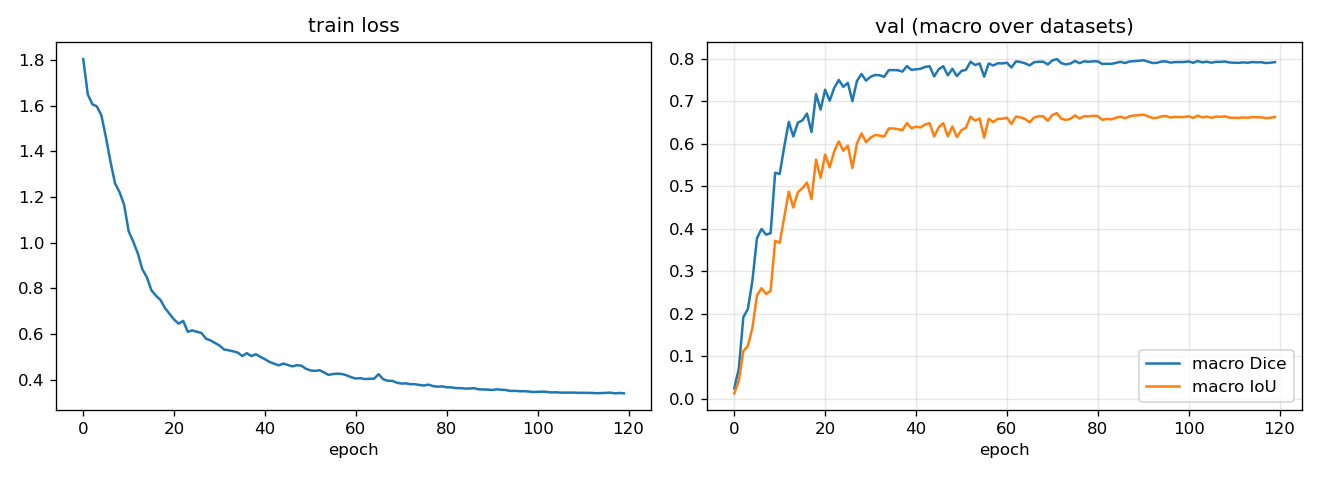
\includegraphics[width=0.7\textwidth]{figures/retrain_curves.png}
\caption{Multi-domain retraining curves: training loss and macro-averaged
held-out Dice/IoU across the four out-of-domain datasets (STARE, DRIVE,
microtubules, EPFL EM), 120 epochs.}
\label{fig:retraincurves}
\end{figure}

\begin{figure}[t]
\centering

\includegraphics[width=0.86\textwidth]{figures/retrained_epfl.png}
\caption{Held-out EPFL/Lucchi EM mitochondria: input, ground truth, and the
retrained \method segmentation, across four representative slices from the
guard-gapped held-out block.}
\label{fig:epfl}
\end{figure}

\subsection{Verifying polarity-agnosticity}
We verify the network is genuinely polarity-agnostic on STARE: feeding images
as-is matches an oracle that picks the better of both polarities per image
using ground truth (0.643 vs.\ 0.643). \textbf{We note honestly that we were
not able to recompute the equivalent as-is-vs-oracle comparison for DRIVE,
microtubules, or EPFL within the scope of this study}: the script that
performs it depends on an external dataset cache and a training checkpoint
that are not part of the artifact bundle we evaluated. We report only the
one dataset we could independently verify, and we list completing this
verification across the remaining three datasets as a concrete item for the
camera-ready version rather than asserting it silently held.

\subsection{Sensitivity of the representation to segmentation error}
\label{sec:seg-perturb}
Graph-exactness (Sec.~\ref{sec:method}) guarantees that the stored invariants
describe $G$ faithfully; it says nothing about how faithfully $G$ describes
the specimen when the mask is wrong. Because this section establishes
segmentation as the dominant error source, we measure that dependence
directly rather than asserting it. For each of the 726 organelle images we
take the pipeline's selected mask, degrade it in four controlled ways
(morphological dilation and erosion at radii 1--5\,px, simulating over- and
under-segmentation; random removal of 5--40\% of connected components,
simulating detection misses; and random flips within a 1--3\,px band of the
boundary, simulating noisy mask edges), rebuild the graph from each degraded
mask through the pipeline's own construction, and record the relative error
of the stored invariants against the unperturbed graph, indexed by the
degraded mask's Seg-IoU against ground truth
(Fig.~\ref{fig:segperturb}; 13{,}068 degraded encodes; the baseline masks
here average Seg-IoU 0.870, i.e.\ the learned-segmenter operating point).

Three findings. First, $\beta_0$ is robust in a wide plateau and then fails
abruptly: pooling the mask-shape perturbations, median $|\Delta\beta_0|$ is
\emph{zero} for degraded masks down to Seg-IoU $\approx 0.50$ and jumps to
$20\%$ in the 0.30--0.50 range. \textbf{The 10\%-error threshold for
$\beta_0$ therefore sits at Seg-IoU $\approx 0.5$}---which is not an
abstract boundary: the classical cascade's actual operating point ($0.489$,
Sec.~\ref{sec:repr}) lies on the cliff edge, while the learned front end
($0.889$) sits deep inside the plateau, giving the segmentation upgrade of
Sec.~\ref{sec:seg-standalone} a second, topological justification beyond
IoU. Second, the invariants are not equally fragile: $\beta_1$ (cycle rank)
is the most sensitive by far---1\,px of boundary noise inflates it by two
orders of magnitude (median $+85\times$ baseline), and even 1\,px dilation
changes it by a median of 33\%---so cycle-rank comparisons across masks of
different provenance should be treated as qualitative. Mean width degrades
gracefully and roughly linearly with morphological perturbation
(median $\approx$30\% at 1\,px of dilation or erosion), as geometry
predicts. Third, component removal produces proportionate, predictable
$\beta_0$ loss (dropping 5--40\% of components changes $\beta_0$ by a median
of 25--50\% while moving width by under 8\%), confirming that the graph
degrades \emph{locally}: losing a
structure removes its subgraph without corrupting the invariants of the
structures that remain. Together these results turn the mask-dependence of
Sec.~\ref{sec:method}'s graph-exactness definition into a measured operating
envelope: above Seg-IoU $\approx 0.5$ the stored $\beta_0$ and width
morphometry can be trusted; the stored cycle rank should be trusted only
when masks come from the same segmenter.

\begin{figure}[t]
\centering

\includegraphics[width=\textwidth]{figures/fig_seg_perturb.png}
\caption{Sensitivity of the stored invariants to segmentation error, on the
726-image organelle set. Each panel degrades the pipeline's selected mask in
a controlled way and plots the median relative error of $\beta_0$ (blue),
cycle rank $\beta_1$ (red) and mean width (green) in the graph rebuilt from
the degraded mask, against that mask's Seg-IoU vs.\ ground truth (x-axis
reversed: degradation increases to the right; y-axis symlog). Dashed line:
10\% error. Dotted verticals: the unperturbed learned-mask operating point
(grey, 0.870) and the classical cascade's (gold, 0.489). $\beta_0$ holds a
zero-error plateau down to Seg-IoU $\approx0.5$ and fails beyond it; cycle
rank is the most fragile invariant, inflated by orders of magnitude under
boundary noise; width degrades gracefully.}
\label{fig:segperturb}
\end{figure}


% =====================================================================
\section{Discussion}\label{sec:discussion}
% =====================================================================
\method treats a curvilinear image as an attributed graph, which unifies
compression, morphometry and topology under one object and makes the geometry
a first-class, queryable artefact. The representation is lossy by design:
full-image fidelity is modest relative to general-purpose codecs
(Sec.~\ref{sec:repr}) because texture and non-curvilinear content are not
modelled, and reconstruction IoU is bounded by segmentation quality.

\subsection{Towards temporal tracking and event detection}
The representation established here is intended as the substrate for a further
question: whether morphological \emph{events} inside living cells can be
detected by monitoring how a structure's graph changes between timepoints,
rather than by tracking pixels. Because \method already exposes connectivity,
$\beta_0$/$\beta_1$ and per-branch morphometry as stored attributes, a
divergence between the graphs of the same structure at two instants is
directly computable on the representation---no re-segmentation, no
re-tracing. Realising this requires a correspondence between graphs across
time, which is where the module below begins.

An unevaluated but functionally complete temporal-tracking module
(\texttt{track.py}, $\sim$550 lines) already exists in the codebase, going
beyond the "scaffolded'' description we previously gave it. It replaces
per-frame skeletonisation---which is degenerate at sub-PSF self-contacts,
where a folded filament's two arms fuse into one blob and the medial axis
collapses to a single short line---with a single arc-length-parameterised 1D
curve per structure, seeded from the best-resolved frame (via graph-diameter
longest-path extraction~\cite{hagberg2008networkx}) and propagated frame-to-frame by optical-flow
advection~\cite{farneback2003} with an inextensibility-constrained snake
refinement, plus a "hybrid geodesic'' selector that falls back to the
propagated curve only when the single-frame skeleton geodesic looks
collapsed. \textbf{We flag explicitly that the module's own internal
comments cite quantitative validation results (e.g.\ "100\% of high-tortuosity
failures are self-fusion'', "100\% rescued'' by temporal propagation) that
reference two experiment scripts not present in the evaluated repository
snapshot}, so we cannot independently verify those specific figures here; we
report the module's existence and design honestly as implemented-but-
unvalidated engineering, and its systematic evaluation (ideally against
manually-tracked ground truth on a live-imaging time series) is deferred to
future work.

\subsection{Limitations}
The external out-of-domain datasets are small (16 training images for
STARE/DRIVE), so their numbers, though leakage-free, are single-split
estimates; the EM result is on correlated slices from one volume with a
guard-gap split. The polarity-agnostic retraining is an
input-representation fix, not a claim of universal segmentation. The
cascade's default segmenter-selection heuristic currently under-uses the more
accurate learned segmenter on the organelle set itself
(Sec.~\ref{sec:seg-standalone})---a limitation of the arbitration logic, not
of the learned segmenter. Segmentation also fails outright on one public
mitochondrial acquisition despite it being in the pipeline's nominal domain
(Sec.~\ref{sec:mito-gen}): acquisition shift within a modality is as
damaging as modality shift, and the single-acquisition training set is the
cause.
The error-guided refinement stage (Sec.~\ref{sec:optimizer}) contributes
nothing to any number reported here: it is enabled, but its residual trigger
is never met on these datasets. It is therefore an untested component rather
than a validated one, and the results should be read as characterising the
skeleton-sampling encoder alone. Finally, the ground-truth-referenced codec
comparison on the annotated out-of-domain datasets (Sec.~\ref{sec:cross-gt})
favours byte-matched JPEG on foreground fidelity: on dense modalities the
structure-proportional payload grows to the point where a general-purpose
codec at the same budget is simply better photometrically, and \method's
case there rests on the structure it exposes and on payloads below JPEG's
byte floor, not on fidelity.

\subsection{Future work}
Natural extensions are 3-D graphs (the underlying medical/biological
structures are frequently volumetric even where we currently process 2-D
slices or projections), systematic validation of the temporal-tracking module
against ground-truth trajectories---for which mitochondrial network tracking
already provides both a target application and an evaluation
protocol~\cite{wang2023mitotnt}---extension of the
background-grid/residual-coding ablation to dense imagery with grid size and
residual quality varied independently,
recalibration of the cascade's segmenter-selection score against
held-out accuracy rather than proxy features, completion of the
oracle-polarity verification on the three remaining out-of-domain datasets,
a polarity- and background-robust ground-truth-referenced reconstruction
metric to replace the organelle Otsu protocol that degenerates on
dark-on-bright imagery (Sec.~\ref{sec:cross-gt}),
a rate--distortion study of the error-guided refinement stage in which the
node budget is deliberately reduced and the residual threshold $\varepsilon$
swept, so that the stage can be evaluated in the regime where it is designed
to act rather than one where it never triggers (Sec.~\ref{sec:optimizer}),
and graph-native downstream models (e.g.\ graph neural networks operating
directly on the stored attributed graph rather than on re-derived features)
for database-searchable microscopy. A further priority is a controlled
reconstruction-quality comparison against our prior compact-representation
systems on a single shared split (Sec.~\ref{sec:prior-quality}), which would
turn the storage-side comparison reported here into a full head-to-head
evaluation.

% =====================================================================
\section{Conclusion}
% =====================================================================
We presented \method, a structural graph representation for curvilinear
microscopy that is compact, analysable and reconstructable in one object. It
extends our prior compact-representation systems---genetic-algorithm-guided
and U-Net-guided key-pixel selection with kernel- and GAN-based
reconstruction~\cite{malakar2025eaai,banerjee2023acpr,banerjee2024gunetpp}---by
replacing an unstructured key-pixel set with an explicit attributed graph
and by turning the segmentation front end those prior systems left as future
work into a first-class object of study. That structural upgrade is
essentially free in storage terms: \method spends the same byte budget as
its predecessors, reallocated from many bare coordinates to few richly
attributed graph nodes (Sec.~\ref{sec:prior-comparison}). \method compresses competitively
with JPEG, WebP and JPEG~2000 at equal bytes on foreground fidelity while
exposing morphometry and graph-exact topology for free, transfers unchanged
across five modalities, and---with a polarity-agnostic multi-domain
segmenter---restores fidelity on out-of-domain vessels, filaments and
electron-microscopy mitochondria. In extending the evaluation for this
journal version we also held the method itself to closer scrutiny than
before: we disambiguated its overlapping IoU and topology metrics, reported
the graph-exact Betti-number topology it has always implied, and surfaced a
segmenter-selection mismatch in our own pipeline as an actionable finding
rather than omitting it. We believe this level of self-scrutiny, alongside
the positive results, is what a representation that asks downstream users to
trust it in place of raw pixels should be held to.

% =====================================================================
\section*{Software and data availability}
% =====================================================================
The encoder/decoder implementation, configuration presets, evaluation
scripts, and the multi-domain and organelle segmenter weights used in this
paper are available at \url{https://github.com/NirwanUiT/Nanograph}. The
726-image organelle dataset is an in-house live-cell mitochondrial
fluorescence-microscopy acquisition that is not yet publicly deposited; STARE~\cite{stare}, DRIVE~\cite{drive} and the
EPFL/Lucchi EM volume~\cite{lucchi} are publicly available from their
respective original sources. No automated regression/unit test suite
currently accompanies the codebase (the existing demo/benchmark entry point
is a CLI script, not a test suite); we record its absence here for completeness.

% ---------------------------------------------------------------------
\section*{Author contributions}

\textbf{Nirwan Banerjee}: conceptualisation, methodology, software,
investigation, data curation, visualisation, writing (original draft).
\textbf{Dilip K. Prasad}: supervision, funding acquisition, writing (review
and editing).

\section*{Competing interests}
The authors declare no competing interests.

\section*{Acknowledgements}
This work was supported by the Research Council of Norway Project (nanoAI,
Project ID: 325741), the H2020 Project (OrganVision, Project ID: 964800),
and the VirtualStain Project (UiT, Cristin Project ID: 2061348).


% ---------------------------------------------------------------------
\bibliographystyle{naturemag}
\bibliography{references}

\end{document}
